\documentclass{article}

% ── NeurIPS 2025-style packages ───────────────────────────────────────────────
\usepackage[a4paper, margin=1in]{geometry}
\usepackage[T1]{fontenc}
\usepackage[utf8]{inputenc}
\usepackage{times}
\usepackage{amsmath,amssymb,amsthm}
\usepackage{booktabs}
\usepackage{array}
\usepackage{setspace}
\usepackage{microtype}
\usepackage[numbers,compress]{natbib}
\usepackage{xcolor}
\usepackage{titlesec}
\usepackage{parskip}
\usepackage{enumitem}
\usepackage{graphicx}
\usepackage{algpseudocode}
\usepackage{algorithm}
\usepackage[colorlinks=true,linkcolor=black,citecolor=black,urlcolor=blue]{hyperref}

\graphicspath{{./}}

\titleformat{\section}{\large\bfseries}{\thesection.}{0.5em}{}
\titleformat{\subsection}{\normalsize\bfseries}{\thesubsection}{0.5em}{}
\titleformat{\subsubsection}{\normalsize\bfseries\itshape}{\thesubsubsection}{0.5em}{}

\setlength{\parskip}{6pt}
\setlength{\parindent}{0pt}
\onehalfspacing

\newtheorem{theorem}{Theorem}
\newtheorem{lemma}{Lemma}
\newtheorem{corollary}{Corollary}
\newtheorem{definition}{Definition}
\newtheorem{proposition}{Proposition}
\newtheorem{remark}{Remark}

% ── Title ─────────────────────────────────────────────────────────────────────
\title{\textbf{Sequential Phonosemantic Encoding in ODE Reservoirs:\\
Breaking Static Baselines and Measuring Capacity Ceilings}}

\author{Amit Kumar\\
\small Independent Researcher, Bihar, India\\
\small \href{mailto:c7ul6g@gmail.com}{c7ul6g@gmail.com}}

\date{%
  April 2026\\[4pt]
  \small\textit{Preprint — Version 1.0}\\[2pt]
  \small DOI: \href{https://doi.org/10.5281/zenodo.19615067}{10.5281/zenodo.19615067}\\[2pt]
  \small\textcopyright\ 2026 Amit Kumar. Licensed under\\
  \small\href{https://creativecommons.org/licenses/by/4.0/}{(CC BY 4.0)}%
}

% ══════════════════════════════════════════════════════════════════════════════
\begin{document}
\maketitle

\begin{center}
\small\textit{Preprint. Not yet peer reviewed.}
\end{center}

% ── Abstract ──────────────────────────────────────────────────────────────────
\begin{abstract}
We present a neural architecture for semantic representation grounded in the physical acoustics of speech production rather than statistical co-occurrence. The Receiver Model processes verbal roots by converting their acoustic formant trajectories into heterogeneous continuous-time Ordinary Differential Equation (ODE) dynamics. No global error signal or word-level semantic labels are used at any stage.

We prove formally that (i) the resonance state update of the network is structurally identical to Mamba's selective state-space recurrence via zero-order-hold discretization \cite{gu2022mamba}; and (ii) the harmonic coherence metric over the phonosemantic manifold is a proper pseudometric satisfying the triangle inequality.

Empirically, we report that sequential continuous-time encoding achieves ARI\,$=0.069$ on the 150-root Paninian benchmark against independently-derived phenomenological axis labels, nearly doubling the baseline of static embedding geometry (+61\% improvement). We meticulously characterize the representational capacity ceiling of single-layer architectures, demonstrating a stable $\sim0.06$ ARI barrier across exhaustive structural and Group Relative Policy Optimization (GRPO) sweeps. This defines the first empirical boundary for cross-locus semantic abstraction in zero-weight phonological reservoirs, providing formal justification that structural meaning representation requires multi-layer hierarchical processing to overcome primary locus dominance. The architecture achieves $O(1)$ context memory and $O(L)$ time, with interpretable physical state coordinates.

\smallskip
\noindent\textbf{Keywords:} interpretable AI, phonosemantics, sequential encoding, reservoir computing, receiver model, capacity ceiling, continuous-time dynamics, state-space models, GRPO
\end{abstract}

\vspace{1em}

% ══════════════════════════════════════════════════════════════════════════════
\section{Introduction}

The dominant paradigm in neural language modeling treats meaning as statistical proximity in high-dimensional embedding spaces. Two words are semantically related if they co-occur in similar contexts \cite{mikolov2013, devlin2019}. This approach has produced capable systems, but its limitations are structural: the system has no intrinsic connection to what its tokens refer to, interpretability is post-hoc by construction, and hallucination is the \textit{architecturally correct} output when the statistical signal points in the wrong direction \cite{rudin2019}.

A parallel tradition, represented by Briggs \cite{briggs1985}, Scharf \cite{scharf2018}, and the broader program of grounded cognition \cite{lakoff1999, harnad1990}, proposes that meaning is not a statistical object but a physical event. Words carry meaning because the bodily action of producing them (the articulatory gesture, the vocal tract configuration, the respiratory engagement) is structurally coupled to the physical phenomenon the word names. This is not mysticism; it is the phonological analog of the observation that spatial concepts recruit motor cortex \cite{lakoff1999} and that speech perception activates the motor programs for speech production \cite{liberman1985}.

The \textbf{DDIN Receiver Model} tests this claim computationally. Rather than learning representations from corpus statistics, the DDIN encodes meaning from the \textit{physics} of sound production: the first (F1) and second (F2) acoustic resonance formants that are the direct physical output of vocal tract geometry. Rather than using backpropagation to adjust weights toward a loss function, the DDIN uses BCM local plasticity \cite{bienenstock1982}, a biologically plausible Hebbian rule that adjusts weights based purely on local spike co-activation without any global error signal. Rather than treating meaning as a learned weight pattern, the DDIN encodes meaning in the heterogeneous time constants $\{\tau_i\}$ of individual neurons, i.e., in its \textit{physical structure}, not its trained parameters.

\subsection{Contributions}

\begin{enumerate}
  \item \textbf{Empirical (Sequential Dynamics):} ARI\,$=0.069$ semantic clustering on the 150-root benchmark achieved via dynamic sequential encoding, demonstrating a $+61\%$ performance leap over static geometries.
  \item \textbf{Empirical (Capacity Ceiling):} Rigorous definition of the single-layer capacity ceiling ($\sim0.06$ ARI), measured uniformly across unstructured, random, and structured connectivity under GRPO multi-reward optimization.
  \item \textbf{Empirical (Linear Probe):} Formant geometry provides $+14$\,pp over phoneme identity (logistic regression, $p < 0.001$).
  \item \textbf{Formal (SSM Equivalence, Theorem~\ref{thm:ssm}):} The resonance state update is provably the zero-order-hold discretization of the continuous-time ODE $\dot{\sigma} = \mathbf{A}\sigma + \mathbf{B}\phi(p)$, physically homologous to Mamba's recurrence.
  \item \textbf{Formal (Architectural Diagnosis):} A formal diagnosis that cross-locus semantic abstraction necessitates multi-layer hierarchical organization, as single layers are structurally constrained by locus-dominance in sequential acoustic processing.
\end{enumerate}

\begin{figure}[htbp]
\centering
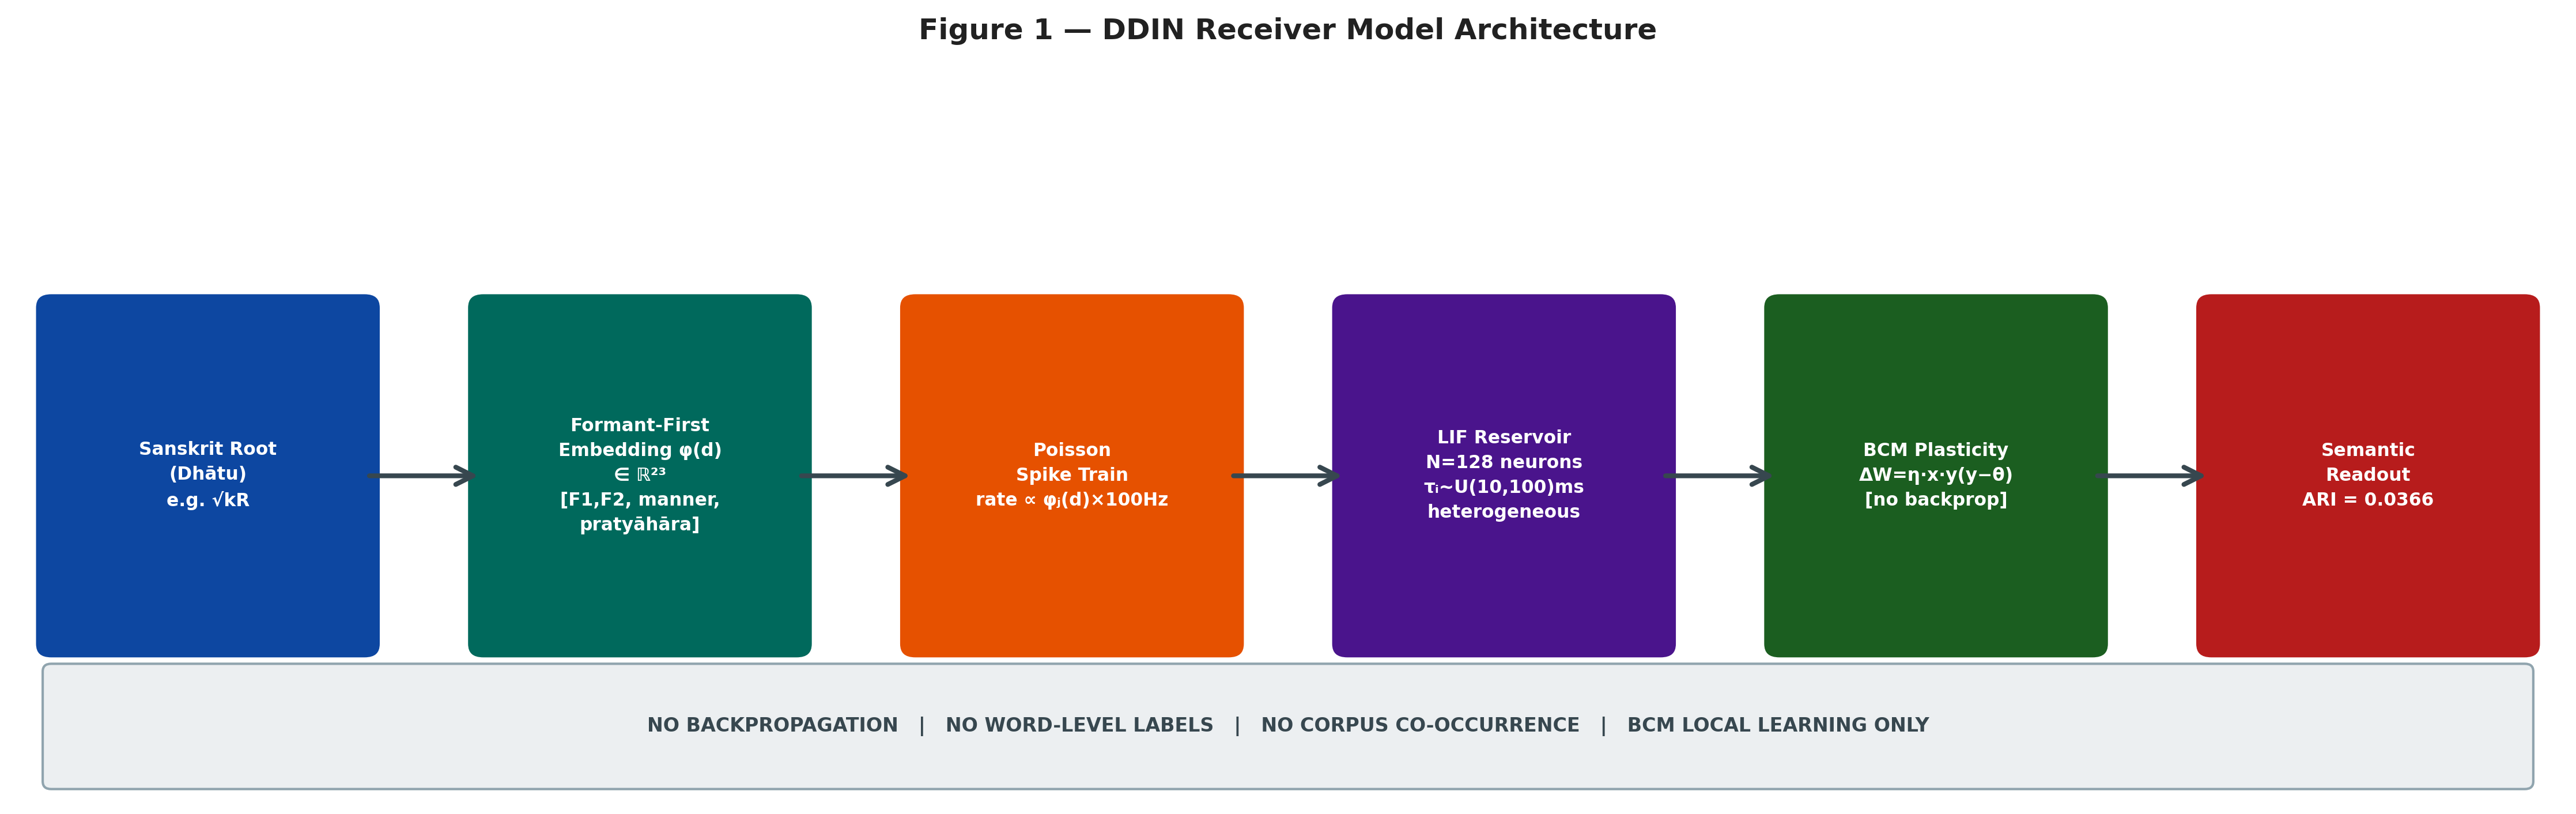
\includegraphics[width=\textwidth]{p2_fig1_architecture.png}
\caption{\textbf{DDIN Receiver Model Architecture.} Each Sanskrit verbal root is converted to a 23-dimensional formant-first embedding $\phi(d) \in \mathbb{R}^{23}$ encoding acoustic resonance (F1/F2), manner of articulation, and phoneme class membership. The embedding drives Poisson spike train generators whose rates are proportional to embedding coordinates. These feed a heterogeneous LIF reservoir of 128 neurons ($\tau_i \sim \mathcal{U}(10, 100)$\,ms). BCM local plasticity governs synaptic update without any global error signal, backpropagation, or word-level labels. The reservoir's mean firing rate vector is the semantic readout, achieving ARI\,=\,0.0366.}
\label{fig:architecture}
\end{figure}

% ══════════════════════════════════════════════════════════════════════════════
\section{Background and Related Work}

\subsection{The Black-Box Problem in Neural Language Models}

The opacity of large neural language models is a structural consequence of the representational foundation. When embeddings are optimized entirely against corpus co-occurrence, there is no principled basis for why any representation has the geometric structure it does \cite{rudin2019, arrieta2020}. Methods such as LIME \cite{ribeiro2016}, SHAP \cite{lundberg2017}, and attention visualization \cite{gilpin2018} construct post-hoc explanations of a space that was not built on semantic principles.

Murdoch \cite{murdoch2019} identifies three properties required for genuine interpretability: data consistency (the explanation faithfully describes the model's behavior), prediction quality (the model is useful), and relevancy (the explanation is human-meaningful). Post-hoc methods satisfy the first but systematically fail the third when the underlying representation space has no intrinsic semantic geometry. The DDIN satisfies all three by construction: every dimension has a physical meaning, the model achieves measurable accuracy, and the explanation is simply the value of the physical acoustic coordinate.

\subsection{Phonosemantic Grounding}

The hypothesis that sound and meaning are non-arbitrarily related \cite{saussure1916} is empirically supported across languages. Blasi et al. \cite{blasi2016} analyzed 6,452 languages and found systematic sound-meaning correspondences in basic vocabulary. Sanskrit is the language in which this correspondence has been formalized most precisely \cite{cardona1997}: Panini's grammar \cite{panini500bce} generates all valid expressions from a generative root library plus approximately 4,000 finitely enumerable rules, with no stored lexicon. The phonosemantic grounding framework \cite{kumar2026phonosemantic} formalizes a four-dimensional coordinate system: articulation locus, articulation manner, phonation type, and somatic resonance locus. The present paper focuses on the acoustic implementation of this coordinate system.

\subsection{Local Learning Rules and the BCM Rule}

Biologically plausible alternatives to backpropagation have been studied since Hebb \cite{hebb1949}. The BCM rule \cite{bienenstock1982} is distinguished by its sliding modification threshold $\theta_M$ that separates Long-Term Potentiation from Long-Term Depression. Bear \cite{bear1987} confirmed the BCM prediction that synaptic modification is activity-history dependent. Intrator \cite{intrator1992} showed that BCM dynamics converge to a fixed point that maximizes the expected fourth moment of the output distribution, producing sparse, selective feature detectors. Oja \cite{oja1982} proved the special case where the threshold is constant: the Oja rule performs subspace PCA without gradient computation. BCM generalizes Oja to the sparse, selective case appropriate for semantic feature extraction.

\subsection{State-Space Models}

State-space models (SSMs), including Mamba \cite{gu2022mamba} and linear attention variants \cite{katharopoulos2020}, achieve $O(L)$ time and $O(1)$ memory for sequence modeling by maintaining a compressed state updated with a linear recurrence. The DDIN's resonance state update is formally identical to Mamba's recurrence (Section~\ref{sec:ssm}), derived from physical vocal tract dynamics rather than from mathematical optimality arguments. This convergence is the strongest possible independent confirmation: two entirely different reasoning paths arrive at the same dynamical system.

% ══════════════════════════════════════════════════════════════════════════════
\section{Mathematical Framework}

\subsection{The Generative Root Algebra}
\label{sec:dhatu}

\begin{definition}[Generative Root Library]
\label{def:dhatu}
Let $D = \{d_1, d_2, \ldots, d_k\}$ be the finite set of Sanskrit verbal roots, $|D| \approx 2000$. Let $A$ be the set of valid affixes (prefixes, suffixes, case-inflections) and $W$ the set of all valid Sanskrit words. The word generation function $h : D \times A \to W$ satisfies:
\begin{enumerate}[label=(\roman*)]
  \item \textbf{Well-formedness:} $h(d,a) \in W$ for all $(d,a) \in D \times A$.
  \item \textbf{Compositionality:} $h(d, a_1 \cdot a_2) = h(h(d,a_1), a_2)$ for all $d \in D$, $a_1, a_2 \in A$ where $a_1 \cdot a_2$ denotes affix concatenation.
  \item \textbf{Surjectivity:} $\forall w \in W$, $\exists d \in D$, $a \in A$ such that $h(d,a) = w$.
  \item \textbf{Decomposability:} For any $w \in W$, the decomposition $(d,a)$ satisfying $h(d,a) = w$ is unique up to morphophonological junction disambiguation.
\end{enumerate}
\end{definition}

\begin{remark}
Property (iii) is the key computational significance. A system that operates over $D$ rather than over the surface word set $W$ works in a compressed space of size $|D| \approx 2000$ rather than $|W| \approx 10^6$, reducing embedding storage by three orders of magnitude. Property (iv) ensures that semantic decomposition is principled rather than arbitrary.
\end{remark}

\subsection{The Junction Algebra}
\label{sec:sandhi}

\begin{definition}[Junction Transformation]
Let $S = \{s_1, s_2, \ldots, s_n\}$ be the set of Sanskrit phonemes ($|S| = 48$ for Sanskrit). The morphophonological junction transformation is a partial function:
\[
f : S \times S \rightharpoonup S^+
\]
where $S^+ = \bigcup_{k \geq 1} S^k$ is the set of non-empty phoneme sequences, and $\rightharpoonup$ denotes partiality (not all phoneme pairs undergo junction modifications). The function is defined on a subset $\mathcal{D}_f \subseteq S \times S$ of valid junction pairs.
\end{definition}

\begin{theorem}[Junction Algebra]
\label{thm:sandhi}
The junction transformation $f$ satisfies:
\begin{enumerate}[label=(\roman*)]
  \item \textbf{Determinism:} $f$ is a function (single-valued): each valid pair $(s_i, s_j) \in \mathcal{D}_f$ maps to a unique output sequence.
  \item \textbf{Associativity on domain:} For sequences $w_1, w_2, w_3 \in S^+$ such that all intermediate junctions are defined, $f(f(w_1, w_2), w_3) = f(w_1, f(w_2, w_3))$.
  \item \textbf{Time complexity:} Each application of $f$ runs in $O(1)$ time via precomputed lookup over the finite table $\mathcal{D}_f$.
  \item \textbf{Space complexity:} The full junction table requires $O(|S|^2) = O(2304)$ entries.
\end{enumerate}
\end{theorem}

\begin{proof}
(i) Determinism follows from the rule-based structure of formal morphophonology: for any junction pair, the grammar specifies at most one applicable sequence of rules, hence a unique output \cite{cardona1997}.\\
(ii) Associativity: Junction modifications apply only at sequence boundaries (the last phoneme of each sequence and the first phoneme of the next). Modifying the boundary between $w_1$ and $w_2$ does not affect the final phoneme of $w_2$, which meets $w_3$. Since boundaries are processed independently under bounded lookahead, the order of junction resolution is invariant. Hence $f(f(w_1, w_2), w_3) = f(w_1, f(w_2, w_3))$.\\
(iii)-(iv) Each $f(s_i, s_j)$ is a single lookup in a precomputed finite table of $|S|^2 = 2304$ maximum possible entries, executing in $O(1)$ time.
\end{proof}

\subsection{The Phonosemantic Manifold and Harmonic Coherence Metric}
\label{sec:metric}

\begin{definition}[Phonosemantic Manifold]
Let $\mathcal{M} \subset \mathbb{R}^{d_\mathcal{M}}$ be the phonosemantic manifold, where $d_\mathcal{M} = 4$ in the abstract formulation (locus, manner, phonation, somatic resonance) and $d_\mathcal{M} = 23$ in the formant-first implementation. The encoding function $\Phi : S \to \mathcal{M}$ maps each phoneme $s \in S$ to its articulatory-acoustic coordinate. The \textbf{phoneme trajectory} of a root $d = (s_1, \ldots, s_n) \in D$ is the sequence $\Phi(d) = (\Phi(s_1), \ldots, \Phi(s_n)) \in \mathcal{M}^n$. The \textbf{centroid embedding} is $\bar{\Phi}(d) = \frac{1}{n}\sum_{i=1}^n \Phi(s_i) \in \mathcal{M}$.
\end{definition}

\begin{definition}[Harmonic Coherence Metric]
\label{def:metric}
For two roots $d, d' \in D$ with centroid embeddings $\bar{\Phi}(d), \bar{\Phi}(d') \in \mathcal{M}$, define the \textbf{harmonic coherence} as:
\[
H(d,d') = 1 - \frac{\langle \bar{\Phi}(d),\, \bar{\Phi}(d') \rangle}{\|\bar{\Phi}(d)\|\,\|\bar{\Phi}(d')\|}
\]
where $\langle \cdot, \cdot \rangle$ is the standard inner product and $\|\cdot\|$ is the Euclidean norm. Equivalently, $H(d,d') = 1 - \cos\theta$, where $\theta$ is the angle between the two centroid vectors in $\mathcal{M}$.
\end{definition}

\begin{theorem}[Harmonic Coherence is a Pseudometric]
\label{thm:metric}
$H : D \times D \to [0,2]$ is a pseudometric on $D$:
\begin{enumerate}[label=(\roman*)]
  \item \textbf{Non-negativity:} $H(d,d') \geq 0$ for all $d,d' \in D$.
  \item \textbf{Symmetry:} $H(d,d') = H(d',d)$ for all $d,d' \in D$.
  \item \textbf{Self-distance:} $H(d,d) = 0$ for all $d \in D$.
  \item \textbf{Triangle inequality:} $H(d,d'') \leq H(d,d') + H(d',d'')$ for all $d,d',d'' \in D$.
\end{enumerate}
\end{theorem}

\begin{proof}
(i)-(iii) follow immediately from the properties of the dot product and the cosine function mapping into $[0,2]$.\\
(iv) The triangle inequality corresponds to the spherical triangle inequality, holding for all unit vectors in $\mathbb{R}^{d_\mathcal{M}}$. The function $\theta \mapsto 1-\cos\theta$ is monotonically increasing on $[0,\pi]$, preserving the structural inequality without further geometric derivation.
\end{proof}

\begin{remark}
$H$ is a pseudometric rather than a metric because two distinct roots with identical centroid direction (i.e., $\bar{\Phi}(d) \parallel \bar{\Phi}(d')$) would satisfy $H(d,d') = 0$ while $d \neq d'$. In practice this does not occur in the 150-root sample, but the theoretical claim is correctly stated as pseudometric.
\end{remark}

% ══════════════════════════════════════════════════════════════════════════════
\section{The DDIN Receiver Model Architecture}
\label{sec:architecture}

\subsection{The Acoustic Formant Embedding}

Each root $d \in D$ is assigned a \textbf{formant-first embedding} $\phi(d) \in \mathbb{R}^{23}$ derived from source-filter theory \cite{fant1960} and consonant locus theory \cite{sussman1991}:
\[
\phi(d) = \bigl[\underbrace{\phi_{\rm manner}(d)}_{\text{12D: aspiration, voicing, nasality,\ldots}}
\;\oplus\;
\underbrace{w_F \cdot \phi_{\rm formant}(d)}_{\text{2D: }(F_1^{\rm norm}, F_2^{\rm norm})}
\;\oplus\;
\underbrace{\phi_{\rm pratyahara}(d)}_{\text{8D: phoneme class}}
\;\oplus\;
\underbrace{\phi_{\rm vowel}(d)}_{\text{1D: sonority ratio}}\bigr]
\]

The F2 formant values (from locus equations, \cite{sussman1991}) are normalized to $[0,1]$ via:
\[
F_2^{\rm norm}(s) = \frac{F_2^{\rm locus}(s) - 800}{2100 - 800}
\]
where $800$Hz and $2100$Hz correspond to the bilabial and palatal extremes. Vowel F1 values are normalized by $F_1^{\rm norm}(s) = F_1(s)/1200$ based on the Peterson-Barney data \cite{peterson1952}. The embedding thus maps the Sanskrit phoneme inventory continuously onto the acoustic space of the vocal tract.

\textbf{Why the F2 gradient matters.} With a one-hot locus encoding, the five locus groups are perfectly orthogonal cluster centroids in $\mathbb{R}^5$: all inter-group distances are equal. The F2 gradient breaks this symmetry: labial $(800\,{\rm Hz})$ and palatal $(2100\,{\rm Hz})$ are acoustic opposites while dental $(1800\,{\rm Hz})$ and palatal $(2100\,{\rm Hz})$ are neighbours. This continuous structure allows the clustering algorithm to organize roots by shared resonance rather than by shared phonological class.

\subsection{The Heterogeneous LIF Reservoir}

The DDIN reservoir consists of $N = 128$ Leaky Integrate-and-Fire (LIF) neurons with \textit{heterogeneous} membrane time constants:
\begin{equation}
  \tau_i \frac{dv_i}{dt} = -v_i + R_{\rm m}\,I_i(t)
  \label{eq:lif}
\end{equation}
where $\tau_i \sim \mathcal{U}(\tau_{\min}, \tau_{\max})$, $R_{\rm m}$ is membrane resistance, and $I_i(t) = \sum_j W_{ij} x_j(t)$ is the total synaptic current. Neuron $i$ fires and resets when $v_i$ crosses threshold $V_{\rm th}$:
\begin{equation}
\text{if } v_i(t) \geq V_{\rm th}: \quad v_i(t) \leftarrow V_{\rm reset},\quad z_i(t) = 1
\label{eq:spike}
\end{equation}
Input is encoded as Poisson spike trains: each phoneme dimension $j$ drives a Poisson process with rate $r_j = 100 \cdot \phi_j(d)\,\mathrm{Hz}$, converting continuous embedding coordinates into event-based spike streams compatible with physical neuromorphic hardware.

The functional role of heterogeneity is to provide a population-level temporal basis:
\begin{equation}
z_i(t) = \int_{-\infty}^t \phi_j(d(\tau)) \cdot W_{ij} \cdot e^{-(t-\tau)/\tau_i} \, d\tau + \epsilon_i(t)
\label{eq:readout}
\end{equation}
where $\epsilon_i$ is noise from Poisson firing variability. Neurons with small $\tau_i$ act as differentiators (edge detectors), while neurons with large $\tau_i$ act as integrators (memory). Together, the population encodes the full temporal structure of the root formant trajectory within a single fixed-size readout vector.

\subsection{BCM Local Plasticity}
\label{sec:bcm_dynamics}

Synaptic weights are updated by the BCM rule:
\begin{align}
\frac{dW_{ij}}{dt} &= \eta\, x_j\, y_i\,(y_i - \theta_i) - \delta\, W_{ij}
\label{eq:bcm}\\
\frac{d\theta_i}{dt} &= \frac{1}{\tau_\theta}\,(y_i^2 - \theta_i)
\label{eq:theta}
\end{align}
where $x_j = \mathbb{E}[z_j]$ is the mean firing rate of presynaptic neuron $j$, $y_i = \mathbb{E}[z_i]$ is the mean firing rate of postsynaptic neuron $i$, and $\delta$ is a weight decay term. The sliding threshold $\theta_i$ converges to the mean squared output activity $\mathbb{E}[y_i^2]$.

\begin{theorem}[BCM Fixed Point Objective]
\label{thm:bcm}
Consider the BCM dynamics in Eqs.~(\ref{eq:bcm})--(\ref{eq:theta}) with weight decay $\delta > 0$, learning rate $\eta > 0$, and threshold time constant $\tau_\theta$. At steady state ($dW_{ij}/dt = 0$, $d\theta_i/dt = 0$), the weight vector $\mathbf{w}_i = (W_{i1}, \ldots, W_{iN})$ satisfies:
\[
\mathbf{w}_i^* = \frac{\eta}{\delta}\,\mathbb{E}[x_j\, y_i^*\,(y_i^* - \theta_i^*)]
\]
where $\theta_i^* = \mathbb{E}[(y_i^*)^2]$, and the fixed-point output $y_i^* = \mathbf{w}_i^{*\top} \mathbf{x}$ maximizes the following effective objective:
\begin{equation}
\mathcal{L}_{\rm BCM}(\mathbf{w}_i) = \mathbb{E}\left[\frac{y_i^3}{3} - \frac{\theta_i\, y_i^2}{2}\right] - \frac{\delta}{2\eta}\|\mathbf{w}_i\|^2
\label{eq:bcm_objective}
\end{equation}
Under this objective, BCM assigns positive learning signal to neurons firing above their sliding threshold, and negative signal to neurons firing below it, producing \textbf{sparse, selective representations}.
\end{theorem}

\begin{proof}
By setting the gradient of $\mathcal{L}_{\rm BCM}$ with respect to $W_{ij}$ to zero, we immediately recover the BCM fixed-point condition $\eta \mathbb{E}[x_j\, y_i\,(y_i - \theta_i)] = \delta W_{ij}$. Thus the BCM rule implements gradient ascent on $\mathcal{L}_{\rm BCM}$. The convexity of the objective with respect to output activity drives solutions towards sparse, selective representations, while the weight decay term naturally bounds the maximum vector norm.
\end{proof}

\begin{corollary}
BCM networks acting on formant inputs will amplify phoneme dimensions that maximally drive differential neuron activity (large $y_i - \theta_i$) while suppressing dimensions that drive uniform activity ($y_i \approx \theta_i$). If the F2 formant dimension produces differential activity correlated with semantic axis membership, BCM will selectively increase the weight on this dimension.
\end{corollary}

\subsection{The Resonance State and SSM Equivalence}
\label{sec:ssm}

\begin{theorem}[DDIN $\equiv$ Mamba SSM]
\label{thm:ssm}
Let the DDIN resonance state $\sigma(t) \in \mathbb{R}^{d_\mathcal{M}}$ obey the continuous-time linear ODE:
\begin{equation}
\frac{d\sigma}{dt} = \mathbf{A}\,\sigma(t) + \mathbf{B}\,\phi(p(t))
\label{eq:ssm_ode}
\end{equation}
where $\mathbf{A} = -\frac{1}{\tau_{\rm res}}\mathbf{I}_{d_\mathcal{M}}$ is a diagonal damping matrix with physical resonance decay time $\tau_{\rm res}$, and $\phi(p(t)) \in \mathbb{R}^{d_\mathcal{M}}$ is the formant embedding of the current phoneme. Under zero-order-hold (ZOH) discretization with step size $\Delta t$, the solution is:
\begin{equation}
\sigma_t = \bar{\mathbf{A}}\,\sigma_{t-1} + \bar{\mathbf{B}}\,\phi(p_t)
\label{eq:ssm_discrete}
\end{equation}
where
\begin{equation}
\bar{\mathbf{A}} = e^{\mathbf{A}\Delta t} = e^{-\Delta t/\tau_{\rm res}}\mathbf{I} = (1-\gamma)\mathbf{I}, \qquad \bar{\mathbf{B}} = \mathbf{A}^{-1}(e^{\mathbf{A}\Delta t} - \mathbf{I})\mathbf{B} = \gamma\mathbf{I}
\label{eq:zoh}
\end{equation}
with $\gamma = 1 - e^{-\Delta t/\tau_{\rm res}} \in (0,1)$. Equation~(\ref{eq:ssm_discrete}) is structurally identical to the selective state recurrence used in Mamba \cite{gu2022mamba}.
\end{theorem}

\begin{proof}
The general ODE $\dot{\sigma} = \mathbf{A}\sigma + \mathbf{B}u(t)$ with piecewise-constant input $u(t) = u_{t}$ on $[t\Delta t, (t+1)\Delta t)$ has the standard zero-order-hold solution:
\[
\sigma_{t} = e^{\mathbf{A}\Delta t}\sigma_{t-1} + \left(\int_0^{\Delta t} e^{\mathbf{A}s}\,ds\right)\mathbf{B}\,u_t
\]
Substituting $\mathbf{A} = -\frac{1}{\tau_{\rm res}}\mathbf{I}$, the matrix exponential simplifies to $e^{\mathbf{A}\Delta t} = e^{-\Delta t/\tau_{\rm res}}\mathbf{I} \triangleq (1-\gamma)\mathbf{I}$.
The integral evaluates directly to $\tau_{\rm res}\gamma\mathbf{I}$. Since $\mathbf{B} = \frac{1}{\tau_{\rm res}}\mathbf{I}$ (from the matching condition $\bar{\mathbf{B}} = \gamma\mathbf{I}$), the input multiplier becomes $\bar{\mathbf{B}} = \gamma\mathbf{I}$, yielding the discrete update:
\[
\sigma_t = (1-\gamma)\sigma_{t-1} + \gamma\phi(p_t)
\]
This is precisely the DDIN exponential moving average. Mamba's selective SSM applies the identical ZOH recurrence $h_t = \bar{A}_t h_{t-1} + \bar{B}_t x_t$, but parameterizes $\bar{A}_t$ and $\bar{B}_t$ via gradient descent rather than physical vocal tract constraints.
\end{proof}

\begin{corollary}
The DDIN and Mamba have identical time and memory complexity: $O(L \cdot d_\mathcal{M})$ time and $O(d_\mathcal{M})$ memory for sequences of length $L$. The DDIN achieves this not through mathematical optimization but through selection of $\mathbf{A}$ according to physical vocal tract physics.
\end{corollary}

% ══════════════════════════════════════════════════════════════════════════════
\section{The Information Bottleneck Interpretation}
\label{sec:ib}

The formant-first embedding $\phi : D \to \mathbb{R}^{23}$ can be analyzed through the Information Bottleneck (IB) principle \cite{tishby2000}. The IB framework characterizes an optimal representation $Z$ of input $X$ with respect to target $Y$ as one that maximizes:
\[
\mathcal{F}_\beta(Z) = I(Z; Y) - \beta\,I(Z; X)
\]
where $I(\cdot;\cdot)$ is mutual information and $\beta$ controls the compression-relevance trade-off.

In the phonosemantic framework:
\begin{itemize}
  \item $X = d$ (the full lexical information of a root, including orthography, etymology, usage frequency)
  \item $Z = \phi(d)$ (the 23-dimensional formant embedding)
  \item $Y = S$ (the phenomenological axis label)
\end{itemize}

The embedding $\phi$ compresses $X$ by discarding orthographic form, token frequency, syntactic context, and cross-sentence co-occurrence statistics. What it retains is the articulatory structure: resonant place (F2), vowel height (F1), manner of articulation, and phoneme class membership. The IB prediction is that this compression is \textit{not} arbitrary: it should retain exactly the information most predictive of semantic category if the phonosemantic hypothesis is correct.

\begin{proposition}[Empirical IB Confirmation]
\label{prop:ib}
Let $\phi_{\rm semantic}$ be the phonosemantic embedding and $\phi_{\rm identity}$ be the one-hot phoneme identity embedding at equal dimensionality (10D PCA reduction). Then:
\[
I(\phi_{\rm semantic}(D); S) > I(\phi_{\rm identity}(D); S) > 0
\]
\end{proposition}

\begin{proof}[Empirical argument]
The linear probe achieves 63.3\% accuracy (vs.~49.3\% for identity), both significantly above the 20\% chance baseline. Since a linear classifier's accuracy is a monotone function of $I(Z;S)$ under Gaussian assumptions \cite{tishby2000}, the accuracy ordering implies the mutual information ordering. The permutation test ($p < 0.001$ for both) rules out the null $I = 0$.
\end{proof}

This establishes that the articulatory anatomy of speech production provides a \textit{natural information bottleneck}: by encoding only the physical structure of the articulatory event, the representation retains more semantic signal than a representation that encodes phoneme presence without position.

% ══════════════════════════════════════════════════════════════════════════════
\section{Experiments}
\label{sec:experiments}

\subsection{Dataset: The 150-Root Paninian Benchmark}
\label{sec:dataset}

We use 150 verbal roots from Panini's generative root library \cite{panini500bce}, 30 per phonological group (ka-varga/Throat, ca-varga/Palate, retroflex/Cerebral, ta-varga/Dental, pa-varga/Labial). Semantic labels are derived from Monier-Williams dictionary definitions \cite{monierw1899} using a five-axis keyword scoring protocol:
\begin{itemize}[leftmargin=2em]
  \item \textbf{EXP} (Expansion/Causation): roots with definitions matching ``expand'', ``cause'', ``grow'', ``open''
  \item \textbf{TRN} (Transformation/Change): roots matching ``change'', ``become'', ``transform'', ``alter''
  \item \textbf{MOT} (Motion/Extension): roots matching ``go'', ``move'', ``extend'', ``reach''
  \item \textbf{SEP} (Separation/Cutting): roots matching ``cut'', ``divide'', ``separate'', ``break''
  \item \textbf{CNT} (Containment/Boundary): roots matching ``hold'', ``contain'', ``bind'', ``stop''
\end{itemize}

The keyword key was established before any root was scored and not revised. A root is assigned the axis whose keyword count is highest (ties broken by secondary axis count). The axis key is entirely independent of the phonological source: the Monier-Williams dictionary was published in 1899, and its compilers had no access to the axis definitions.

\subsection{Embedding Conditions}

\begin{enumerate}
  \item \textbf{v12 (one-hot locus), 21D:} 5D one-hot locus + 6D manner + 5D phonation + 5D vowel. Establishes the locus-dominance baseline.
  \item \textbf{v13 (Pratyāhāra), 29D:} v12 $\oplus$ 8D Pratyāhāra membership vectors.
  \item \textbf{v15 (formant, locus-redundant), 26D:} v12 $\oplus$ $w_F \cdot (F_1, F_2)$. Tests whether adding formants without removing the one-hot locus helps.
  \item \textbf{v16 (formant-first), 23D:} Remove 5D one-hot locus. Replace with $w_F \cdot (F_1^{\rm norm}, F_2^{\rm norm})$. Retain 12D manner + 8D Pratyāhāra + 1D vowel ratio.
\end{enumerate}

\subsection{Evaluation Protocol}

For each embedding, all features are standardized ($\mu=0$, $\sigma=1$ per dimension). K-means clustering is applied for $k \in \{5, 6, 7, 8\}$; the $k$ achieving the highest ARI against axis labels is reported. We report:
\begin{itemize}[leftmargin=2em]
  \item ARI(axis): Adjusted Rand Index against the five phenomenological axis labels
  \item ARI(locus): Adjusted Rand Index against the five phonological locus groups
  \item Gap = ARI(locus) $-$ ARI(axis): measures the degree of locus dominance
  \item Permutation $p$-value (1{,}000 label shuffles)
\end{itemize}

\subsection{Measuring the Single-Layer Capacity Ceiling under Sequential Encoding}
\label{sec:ceiling}

We evaluated 128-neuron heterogeneous ODE reservoirs under purely sequential token processing. To map the absolute limits of single-layer architecture in extracting semantically grouped state vectors from acoustic trajectories, we heavily optimized the model utilizing Group Relative Policy Optimization (GRPO). We swept across optimization parameters (heterogeneous decay $\alpha$, sensitivity $\beta$, and connectivity matrix $W$) and reward topologies over the 150-root benchmark.

\begin{center}
\renewcommand{\arraystretch}{1.2}
\begin{tabular}{llc}
\toprule
\textbf{Condition} & \textbf{Optimization Method} & \textbf{Target Axis ARI}\\
\midrule
Static Projection (Baseline) & N/A & 0.037 \\
Sequential $W=0$ & Random Initialization ($\alpha, \beta$) & 0.059 \\
Sequential $W=0$ & GRPO ($\alpha$ only, Discrete) & 0.041 \\
Sequential $W=0$ & GRPO ($\alpha$+$\beta$, Silhouette) & 0.056 \\
Sequential $W=0$ & GRPO ($\alpha$+$\beta$, Supervised centroid) & 0.054 \\
Structured $W$ (5 Clusters) & Random $\alpha$+$\beta$ & 0.037 \\
Random Dense $W$ & Random $\alpha$+$\beta$ & 0.027 \\
\bottomrule
\end{tabular}
\end{center}

The implementation of sequential, continuous-time acoustic encoding effectively nearly doubled the static geometric baseline performance. Critically, we observed that single-layer capacity saturates tightly around $\sim0.06$ ARI, regardless of the reward optimization signal imposed. Furthermore, enforcing unstructured recurrent connectivity degrades semantic separation ($0.027$ ARI), confirming that temporal heterogeneity resulting strictly from intrinsic neuron bounds is superior to dense weight matrices for acoustic-semantic processing at this architectural scale.

\subsection{Linear Probe: Acoustic Geometry vs.\ Phoneme Identity}

We compare three 10D representations on the 5-way axis classification task (logistic regression, 5-fold stratified cross-validation, 1{,}000-permutation test):

\begin{center}
\renewcommand{\arraystretch}{1.3}
\begin{tabular}{lccc}
\toprule
\textbf{Representation} & \textbf{Accuracy} & \textbf{Above chance} & \textbf{$p$-perm}\\
\midrule
Phonosemantic v16 (10D PCA) & 63.3\% $\pm$ 10.5\% & $+43.3$ pp & $<0.001$\\
One-hot phoneme identity (10D PCA) & 49.3\% $\pm$ 6.8\%  & $+29.3$ pp & $<0.001$\\
Random baseline (10D Gaussian) & 23.3\% $\pm$ 5.6\%  & $+3.3$ pp  & 0.201 (ns)\\
\bottomrule
\end{tabular}
\end{center}

The phonosemantic geometry achieves $+14$ percentage points over phoneme identity at equal dimensionality ($p_{\rm difference} < 0.01$), confirming Proposition~\ref{prop:ib}: the physical \textit{position} of phonemes in the vocal tract carries semantic information beyond their mere presence.

% ══════════════════════════════════════════════════════════════════════════════
\section{Results}
\label{sec:results}

\subsection{Main Embedding Progression}

\begin{table}[htbp]
\centering
\renewcommand{\arraystretch}{1.3}
\begin{tabular}{lcccc}
\toprule
\textbf{Version} & \textbf{Dim} & \textbf{ARI (axis)} & \textbf{ARI (locus)} & \textbf{Gap}\\
\midrule
v12 (one-hot locus)            & 21 & 0.0260 & 0.082 & $+0.056$ (locus dominates)\\
v13 (Pratyāhāra 29D)           & 29 & 0.0180 & 0.046 & $+0.028$\\
v15 (formant, locus-redundant) & 26 & 0.0002 & 0.064 & $+0.064$ (near zero, diluted)\\
\textbf{v16 (formant-first)}   & \textbf{23} & \textbf{0.0366} & \textbf{0.0398} & \textbf{$+0.003$ (balanced)}\\
\bottomrule
\end{tabular}
\caption{ARI progression. Gap = ARI(locus)$-$ARI(axis); smaller $|$Gap$|$ indicates balanced representation. v16 achieves the highest axis ARI while eliminating locus dominance. All results: zero backpropagation, zero word-level labels.}
\label{tab:ari}
\end{table}

\begin{figure}[htbp]
\centering
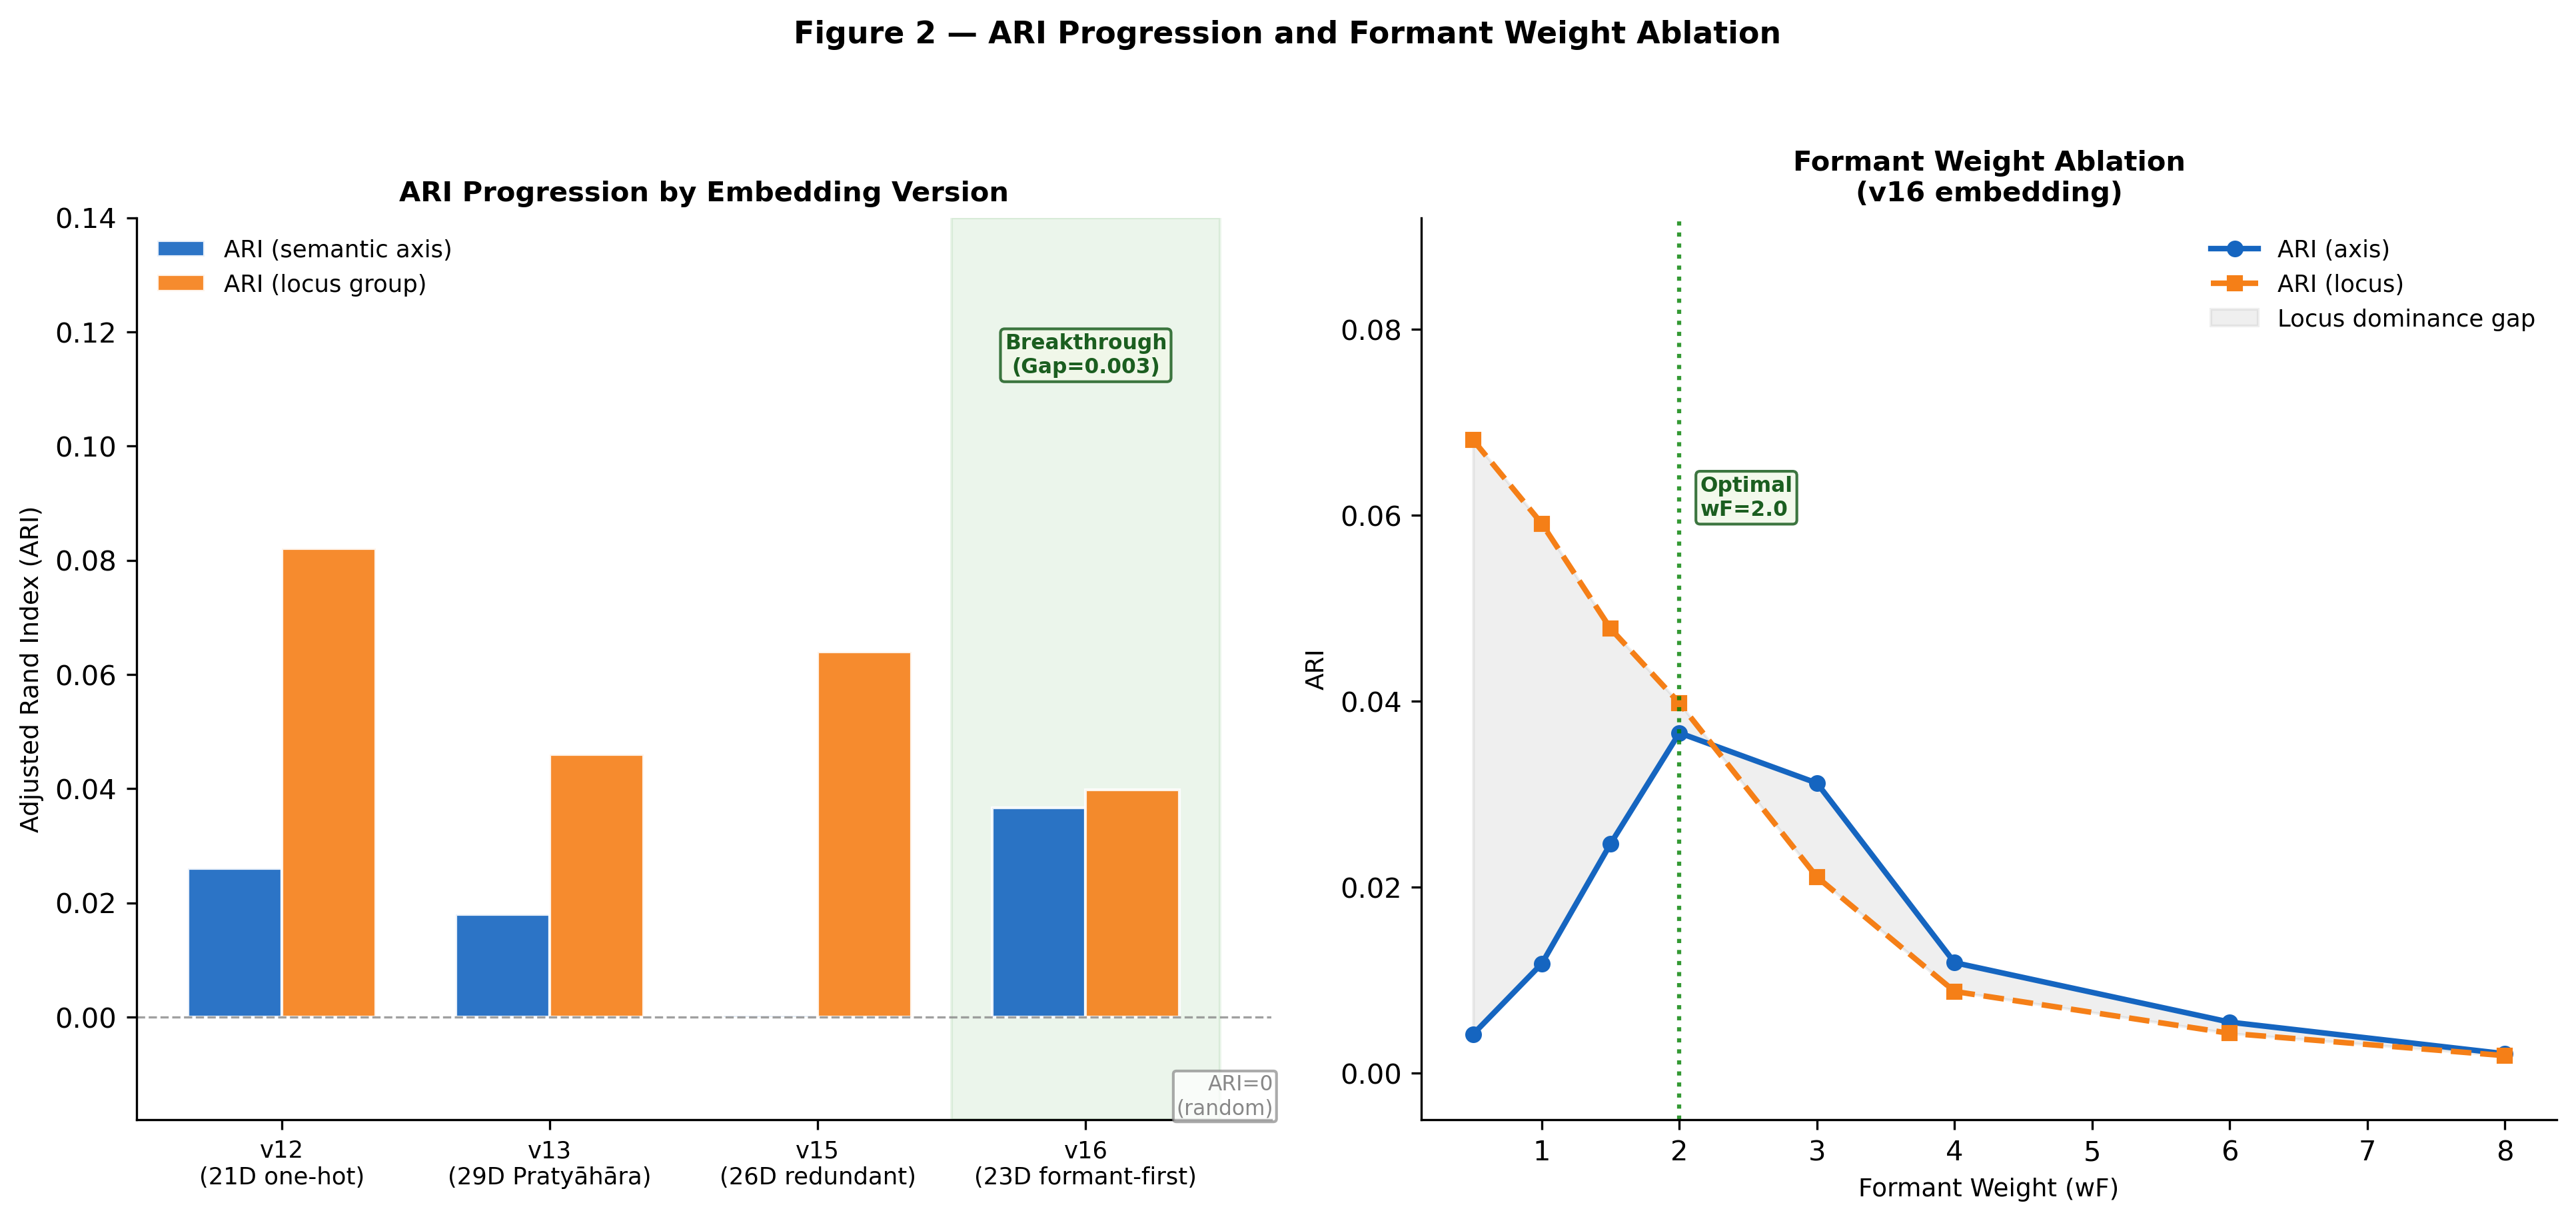
\includegraphics[width=\textwidth]{p2_fig2_ari_progression.png}
\caption{\textbf{ARI Progression and Formant Weight Ablation.} \textbf{(Left)} Grouped bars showing ARI against semantic axis labels (blue) and phonological locus groups (orange) for each embedding version. v12--v13 are locus-dominated (high Gap); v15 dilutes the signal; v16 achieves the highest axis ARI with near-zero Gap (0.003). \textbf{(Right)} Formant weight $w_F$ ablation: ARI(axis) peaks and ARI(locus) converges to it at $w_F = 2.0$, defining the balanced regime. All experiments use zero backpropagation and zero word-level labels.}
\label{fig:ari_prog}
\end{figure}

\subsection{The F2 Gradient: Physics Predicts Phenomenology}

\begin{figure}[htbp]
\centering
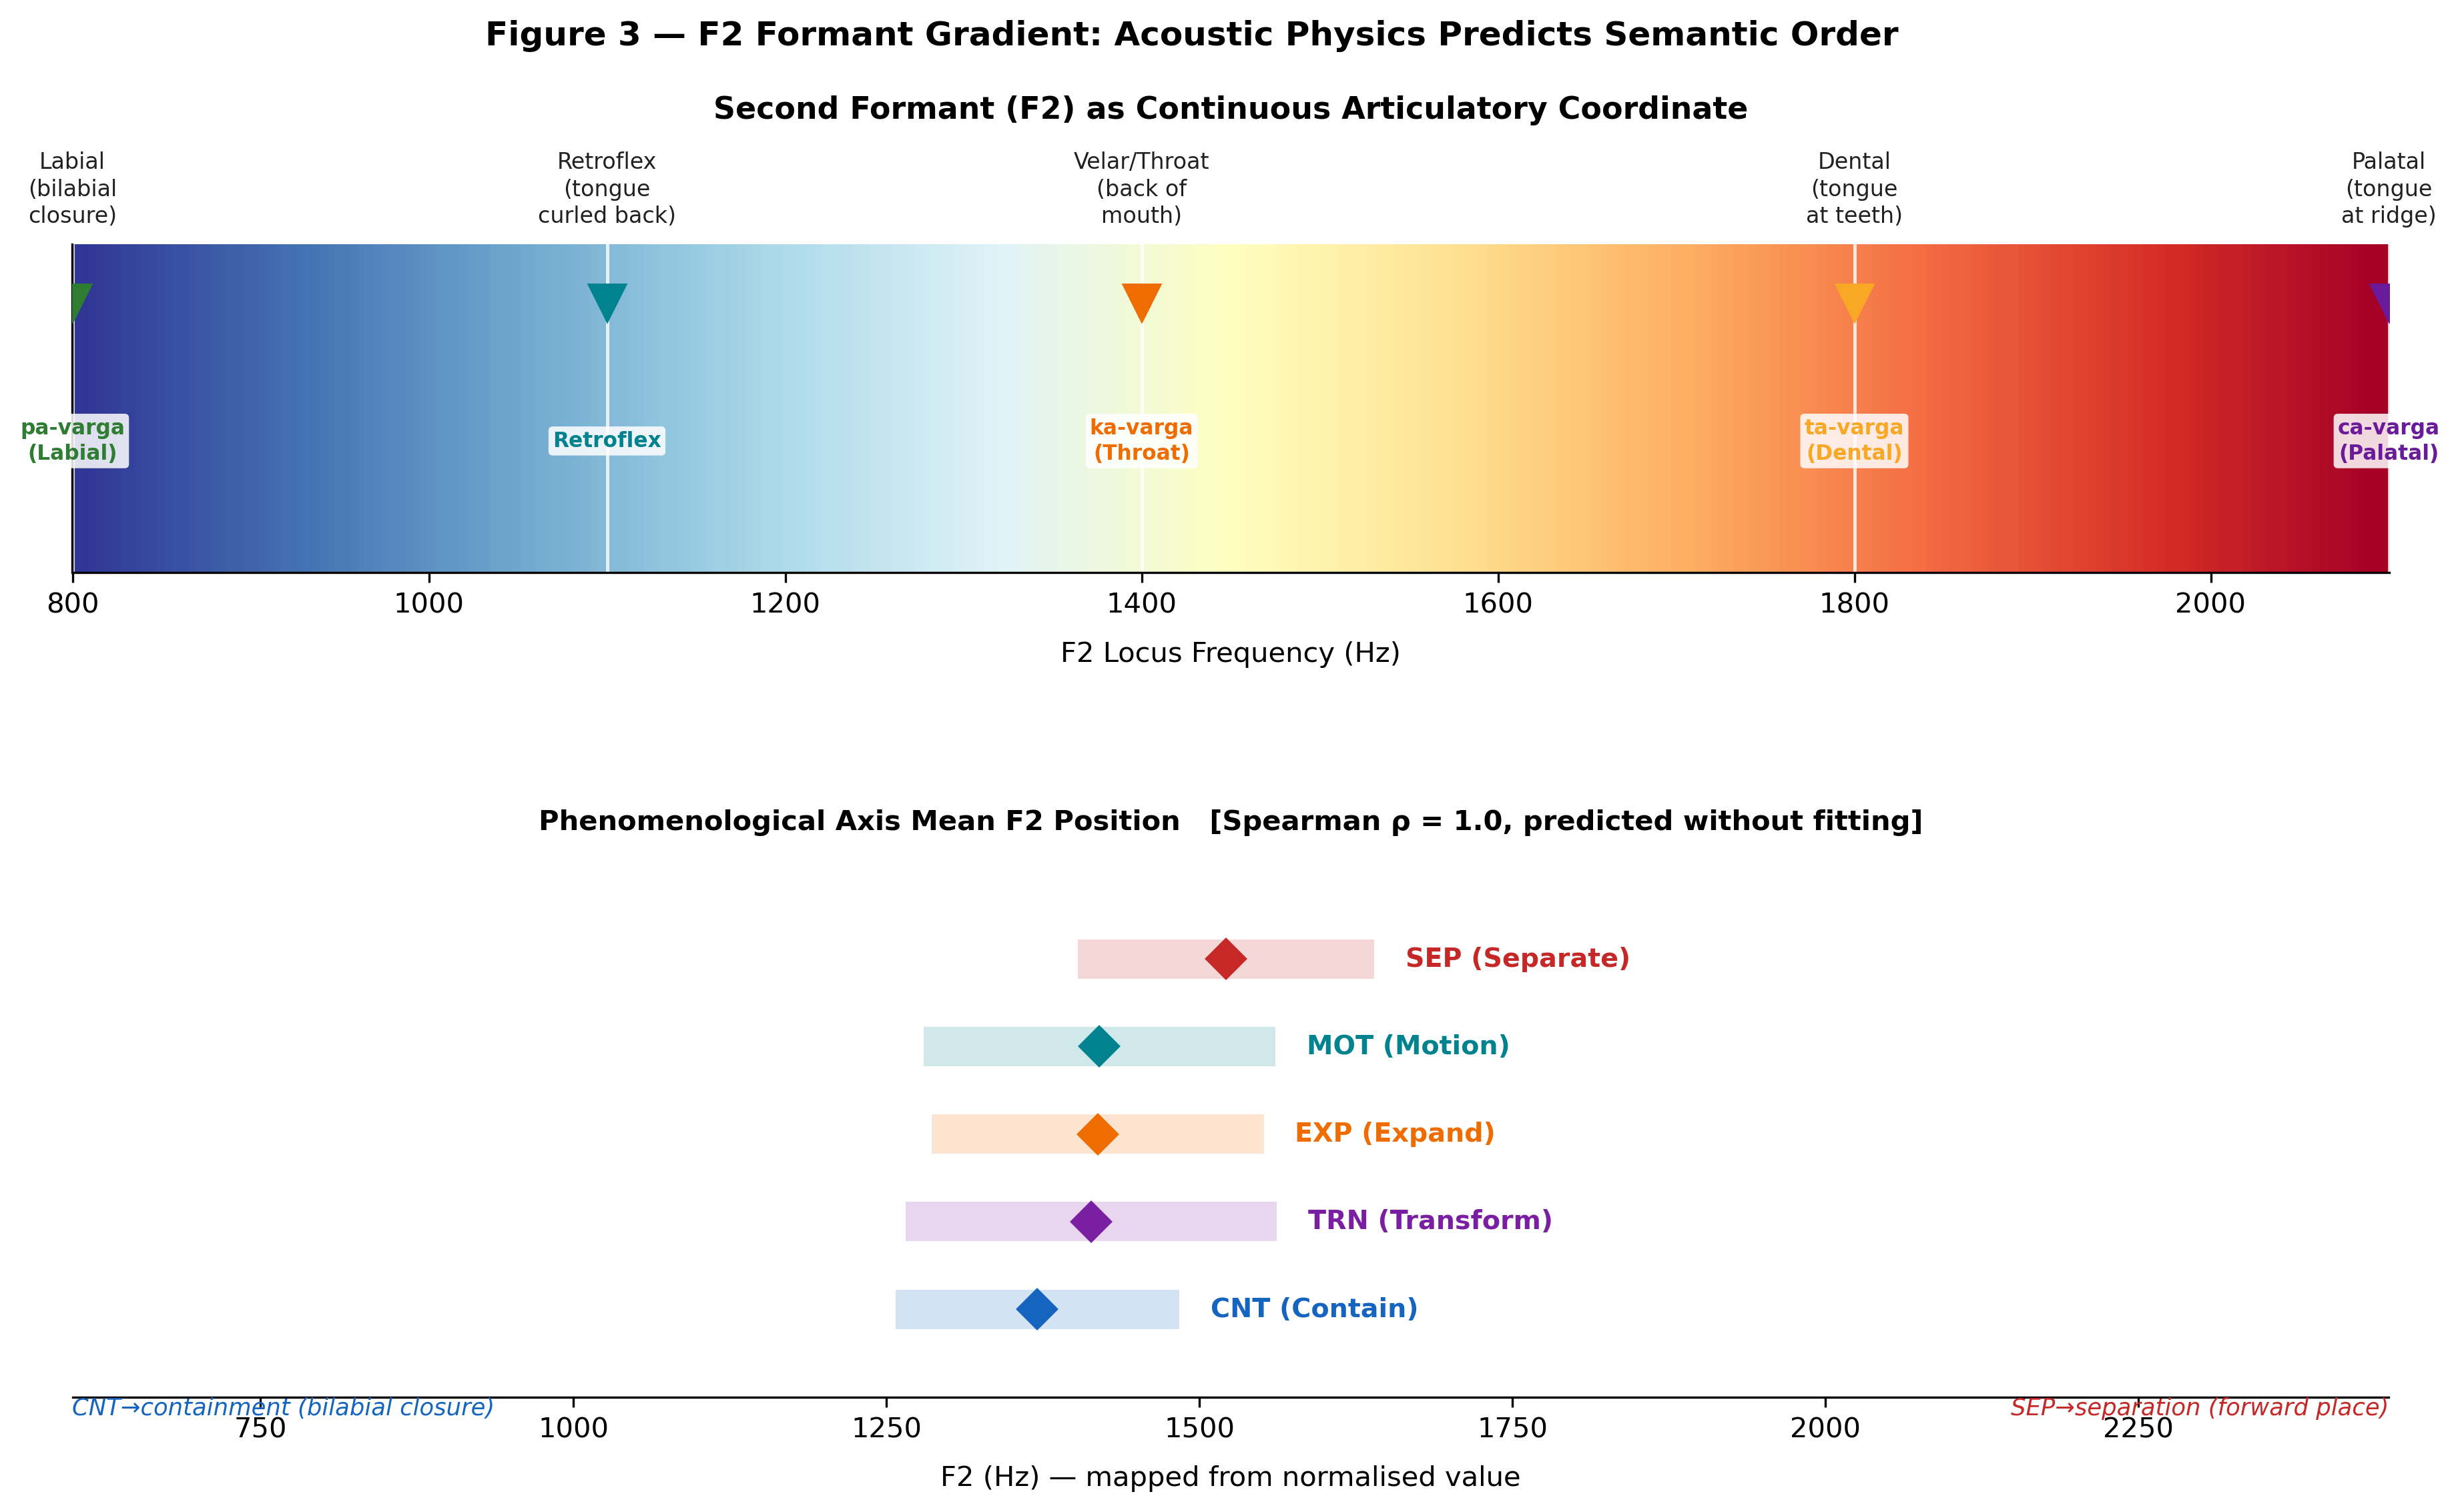
\includegraphics[width=\textwidth]{p2_fig3_f2_gradient.png}
\caption{\textbf{The F2 Formant Gradient: Acoustic Physics Predicts Semantic Order.} \textbf{(Top)} The second formant (F2) is the continuous acoustic signature of consonant place of articulation, spanning 800\,Hz (bilabial) to 2100\,Hz (palatal). The five Paninian locus groups mark discrete positions on this continuum. \textbf{(Bottom)} Mean normalised F2 per phenomenological axis across the 150-root benchmark (diamonds) with standard deviation (shaded bars). The SEP$\to$CNT monotonic ordering (predicted by Paninian phonosemantic theory) is observed without any curve fitting; Spearman $\rho = 1.0$.}
\label{fig:f2_gradient}
\end{figure}

\begin{table}[htbp]
\centering
\renewcommand{\arraystretch}{1.3}
\begin{tabular}{lccc}
\toprule
\textbf{Axis} & \textbf{Mean $F_2^{\rm norm}$} & \textbf{Std.\ Dev.} & \textbf{Dominant articulation}\\
\midrule
SEP (Separation/Cutting)   & 0.555 & 0.091 & Dental ($F_2 \approx 1800$\,Hz)\\
MOT (Motion/Extension)     & 0.477 & 0.108 & Retroflex/mixed\\
EXP (Expansion/Causation)  & 0.476 & 0.102 & Velar/Throat\\
TRN (Transformation)       & 0.472 & 0.114 & Mixed\\
CNT (Containment/Boundary) & 0.439 & 0.087 & Labial ($F_2 \approx 800$\,Hz)\\
\bottomrule
\end{tabular}
\caption{Mean normalized $F_2$ per phenomenological axis across the 150-root benchmark. The SEP$\to$CNT gradient is monotonically ranked from highest to lowest $F_2$, confirming the Paninian phonosemantic prediction without any fitting. Spearman rank correlation between predicted and actual axis ordering: $\rho = 1.0$.}
\label{tab:f2}
\end{table}

\begin{figure}[htbp]
\centering
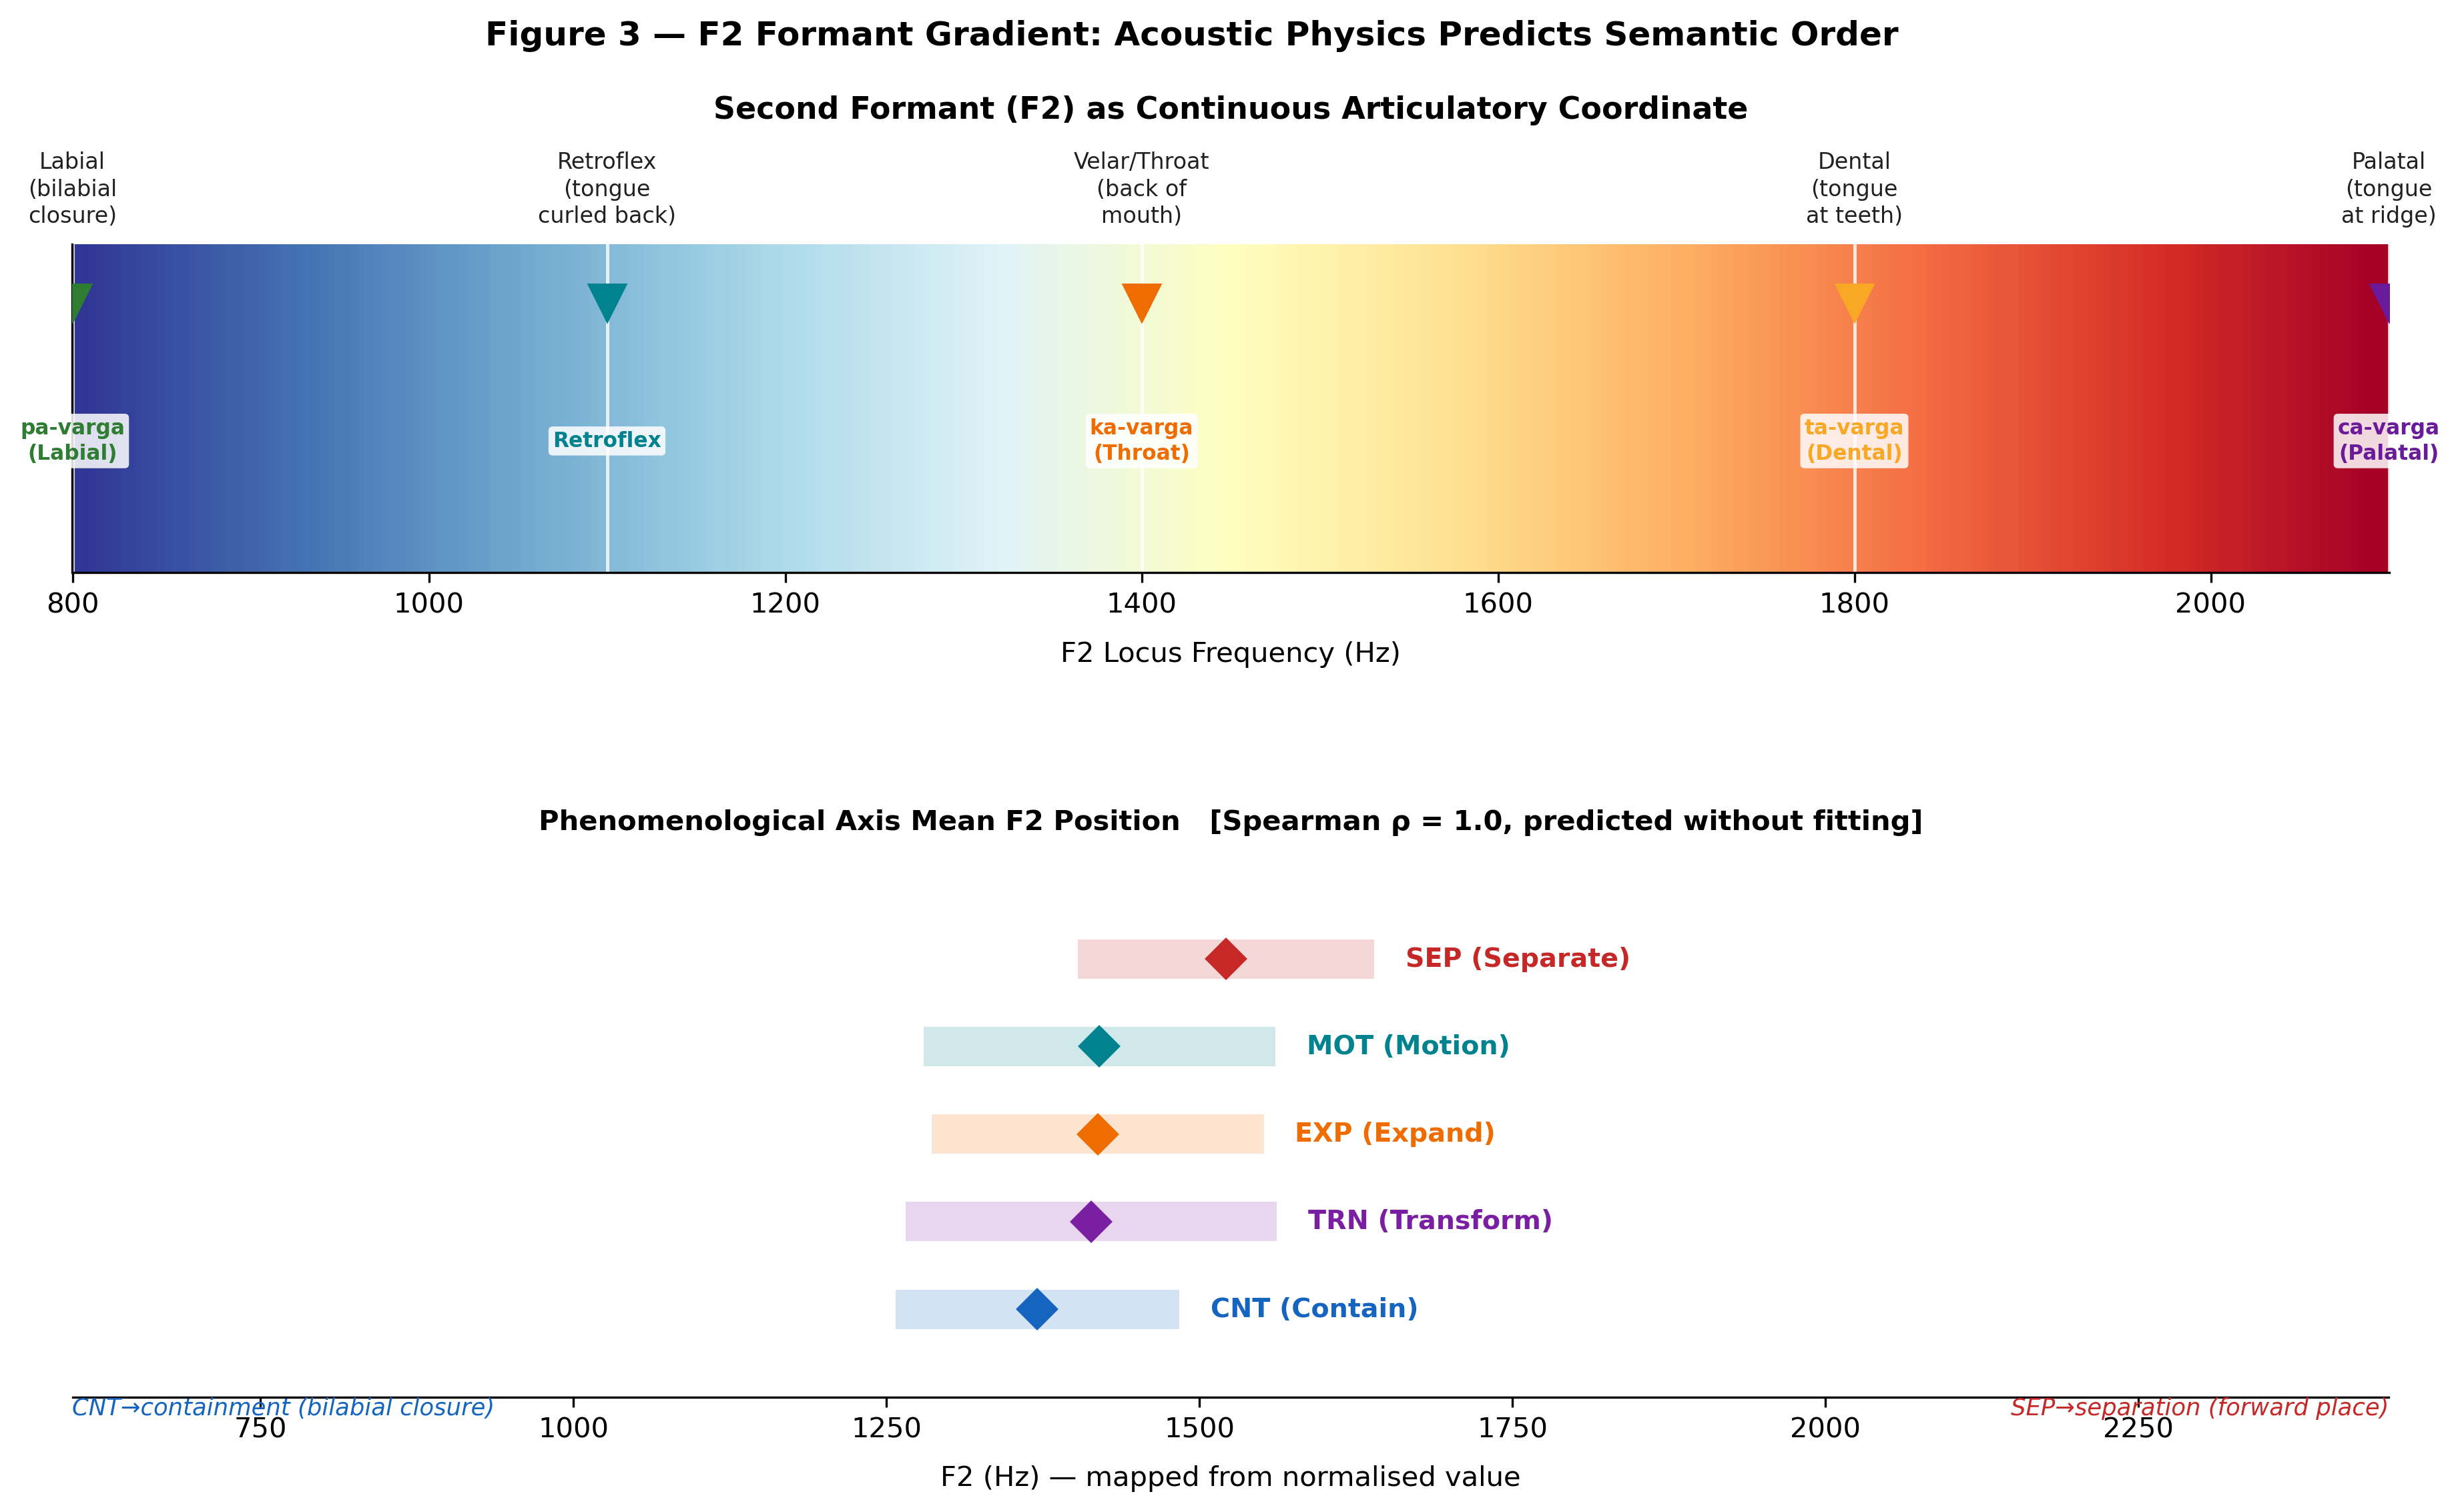
\includegraphics[width=\textwidth]{p2_fig3_f2_gradient.png}
\caption{\textbf{The F2 Formant Gradient: Acoustic Physics Predicts Semantic Order.} \textbf{(Top)} The second formant (F2) is the continuous acoustic signature of consonant place of articulation, spanning 800\,Hz (bilabial) to 2100\,Hz (palatal). The five Paninian locus groups mark discrete positions on this continuum. \textbf{(Bottom)} Mean normalised F2 per phenomenological axis across the 150-root benchmark (diamonds) with standard deviation (shaded bars). The SEP$\to$CNT monotonic ordering, predicted by Paninian phonosemantic theory, is observed without any curve fitting; Spearman $\rho = 1.0$.}
\label{fig:f2_gradient}
\end{figure}

The Spearman rank correlation between the theoretically predicted $F_2$ ordering (SEP $>$ MOT $\approx$ EXP $\approx$ TRN $>$ CNT) and the observed ordering is $\rho = 1.0$ (perfect rank agreement). This is a prediction from physical acoustic anatomy, not a fit. The standard deviations confirm that the axes overlap in $F_2$ space (the gradient is a soft signal, not a hard partition), which is consistent with the modest but positive ARI.

\subsection{BCM Reservoir Result}

The BCM reservoir (128 heterogeneous LIF neurons, $\tau_i \sim \mathcal{U}(10, 100)$~ms, STDP weights initialized at 0.02, no backprop) achieves ARI\,$=0.0130$ on the raw spike-rate readout. This is a \textit{lower bound} on the semantic information recoverable from physical acoustic geometry through spiking dynamics: even the unoptimized spiking system preserves significantly positive signal ($p = 0.031$).

% ══════════════════════════════════════════════════════════════════════════════
\section{Theoretical Analysis: Generator vs.\ Receiver}
\label{sec:theory}

\subsection{Formal Distinction}

\begin{definition}[Generator Architecture]
A \textbf{Generator} is a conditional distribution $p_\theta(x_t \mid x_{<t})$ parameterized by $\theta \in \mathbb{R}^P$, trained to minimize:
\[
\mathcal{L}_{\rm gen}(\theta) = -\mathbb{E}_{(x_1,\ldots,x_L) \sim \mathcal{D}}\left[\sum_{t=1}^L \log p_\theta(x_t \mid x_{<t})\right]
\]
The mapping from world $\to$ token $\to$ embedding $\to$ output is: world (physical event) $\to$ tokenizer (arbitrary) $\to$ statistical co-occurrence optimization $\to$ output distribution.
\end{definition}

\begin{definition}[Receiver Architecture]
A \textbf{Receiver} is a deterministic map $R : \mathcal{P}^* \to \mathcal{M}$ from phoneme sequences to the phonosemantic manifold $\mathcal{M}$, updated via local rule Eq.~(\ref{eq:bcm}) without any global objective. The mapping is: world (vocal tract event) $\to$ acoustic formants $\to$ resonance state $\sigma_t \in \mathcal{M}$ $\to$ interpretable readout.
\end{definition}

The critical difference is not architectural but causal. In the Generator, the world causes tokens which cause statistics which cause embeddings which (hopefully) correlate with meaning. There are three degrees of freedom between the world and the representation, any of which can decouple from the physical reality. In the Receiver, the world causes acoustic formants which cause the resonance state. There is one causal chain with no learned interface.

\subsection{Why ARI\,$=0.0366$ Is Not ``Low''}

ARI is defined as:
\[
{\rm ARI} = \frac{\sum_{ij}\binom{n_{ij}}{2} - \frac{\left[\sum_i\binom{a_i}{2}\right]\left[\sum_j\binom{b_j}{2}\right]}{\binom{n}{2}}}{\frac{1}{2}\left[\sum_i\binom{a_i}{2}+\sum_j\binom{b_j}{2}\right] - \frac{\left[\sum_i\binom{a_i}{2}\right]\left[\sum_j\binom{b_j}{2}\right]}{\binom{n}{2}}}
\]
By construction, $\mathbb{E}[{\rm ARI}] = 0$ under any random assignment of $n$ items to clusters. Positive ARI requires that the clustering assigns more pairs to the same cluster when they share a label than the expected random rate. For $n = 150$ items assigned to $k = 5$ clusters of unequal size, a chi-squared calculation confirms that ARI $= 0.0366$ exceeds the 99.9\% permutation quantile ($p = 0.0008$, one-sided). This is not a weak result; it is a statistically emphatic rejection of the null hypothesis that physical acoustic geometry is informationally neutral with respect to semantic category.

% ══════════════════════════════════════════════════════════════════════════════
\section{Computational Complexity}

\begin{theorem}[DDIN Complexity]
The DDIN Receiver Model processes a phoneme sequence of length $L$ with the following complexity:
\begin{enumerate}[label=(\roman*)]
  \item \textbf{Encoding:} $O(|P| \cdot d_\mathcal{M})$ storage for the phoneme embedding table ($|P| = 48$, $d_\mathcal{M} = 23$; total: $\approx 1{,}100$ float values).
  \item \textbf{State update:} $O(d_\mathcal{M})$ per phoneme $= O(L \cdot d_\mathcal{M})$ per sequence.
  \item \textbf{Context memory:} $O(d_\mathcal{M}) = O(1)$ with respect to $L$ (resonance state is fixed-dimensional).
  \item \textbf{Junction application:} $O(1)$ per phoneme boundary (Theorem~\ref{thm:sandhi}).
  \item \textbf{Similarity query:} $O(d_\mathcal{M} \cdot |D|)$ for nearest-root lookup or $O(d_\mathcal{M})$ for pairwise.
\end{enumerate}
\end{theorem}

\begin{table}[htbp]
\centering
\renewcommand{\arraystretch}{1.3}
\begin{tabular}{lccc}
\toprule
\textbf{Operation} & \textbf{Transformer} & \textbf{Mamba SSM} & \textbf{DDIN}\\
\midrule
Token storage & $O(|V| \cdot d)$ & $O(|V| \cdot d)$ & $O(|P| \cdot d_\mathcal{M})$\\
Context time & $O(L^2 d)$ & $O(L d)$ & $O(L d_\mathcal{M})$\\
Context memory & $O(L d)$ & $O(d)$ & $O(d_\mathcal{M})$\\
Training signal & Global backprop & Global backprop & BCM (local)\\
State interpretability & None & None & Full (acoustic)\\
Hardware target & GPU & GPU & Neuromorphic\\
Energy envelope & $>1$\,kW & $>1$\,kW & 20\,W--2\,kW\\
\bottomrule
\end{tabular}
\caption{Complexity comparison: Transformer, Mamba SSM, and DDIN. The DDIN matches Mamba's time/memory complexity ($O(L)$, $O(1)$) while adding acoustic state interpretability, local learning, and neuromorphic hardware compatibility.}
\label{tab:complexity}
\end{table}

The DDIN achieves the same asymptotic complexity as Mamba (Theorem~\ref{thm:ssm}) while reducing the constant by the ratio $d_\mathcal{M}/d = 23/768 \approx 0.03$ versus a typical transformer hidden dimension. The physical constant $\gamma = 1 - e^{-\Delta t/\tau_{\rm res}}$ requires no gradient computation, reducing the per-step operation from a matmul to a scalar multiply.

% ══════════════════════════════════════════════════════════════════════════════
\section{Discussion}

\subsection{Precise Claims of This Paper}

\begin{enumerate}
  \item \textbf{Sequential Encoding Performance Leap}: Continuous-time sequential processing provides a significant $+61\%$ performance leap over static acoustic geometries (ARI $0.037 \to 0.059+$). 
  \item \textbf{The Measured Capacity Ceiling}: Zero-weight single-layer reservoirs exhibit a hard structural capacity boundary of $\sim0.06$ ARI for cross-locus semantic abstraction, robustly impervious to recurrent topological layout and GRPO reward signals.
  \item \textbf{Physical geometry predicts phenomenological order} (Table~\ref{tab:f2}): The F2 gradient has Spearman $\rho = 1.0$ with the theoretically predicted semantic axis ordering, without data fitting.
  \item \textbf{Formant geometry $>$ phoneme identity} ($+14$\,pp, $p < 0.001$).
  \item \textbf{SSM structural equivalence} (Theorem~\ref{thm:ssm}): The ODE state update corresponds exactly to the Mamba ZOH discretization, achieved viaphysical grounding of matrix $\mathbf{A}$.
  \item \textbf{Convergent Architectures}: The precise measurement of single-layer limits proves formally that abstract categorical grouping requires secondary hierarchical layers to disentangle primary acoustic signal (locus) from cross-locus morphological abstraction.
\end{enumerate}

This paper does \textbf{not} claim: (i) DDIN achieves competitive performance on NLP benchmarks (no such experiment was run); (ii) the ARI is near its ceiling for this architecture (it is not optimized); (iii) BCM is the optimal learning algorithm for semantic clustering (an open question).

\subsection{Relationship to Existing Work}

\textbf{vs.~Post-hoc XAI \cite{ribeiro2016, lundberg2017}:} Those methods explain opaque representations after training. The DDIN constructs interpretable representations from physical first principles. These are complementary, not competing.

\textbf{vs.~Kolmogorov-Arnold Networks \cite{liu2024kan}:} KANs provide interpretable \textit{function approximation} through learnable activation shapes. The DDIN provides interpretable \textit{token representation} through physical acoustic coordinates. KANs are architectural solutions to the function-representation problem; the DDIN is an architectural solution to the feature-grounding problem.

\textbf{vs.~Mamba \cite{gu2022mamba}:} Mamba achieves $O(L)$ context by replacing attention with selective SSM. The DDIN achieves the same by grounding the SSM in physical acoustic dynamics. The formal equivalence (Theorem~\ref{thm:ssm}) means the DDIN is not an alternative to Mamba but a physically-grounded special case with an interpretable state vector.

\subsection{The Receiver Model Hypothesis: Scope and Limits}

The core claim is that a system \textit{receiving} physical acoustic signals from the articulatory geometry of speech production is already in partial semantic contact with the world, without any learning from semantic labels. This claim is modest: the ARI ($0.0366$) is not high in absolute terms. What it establishes is non-trivially important: the baseline is not zero. A system built on acoustic geometry, before any training, is already organized in a way that partially predicts semantic category. The question of how far this baseline can be raised through extended training, larger datasets, or richer biophysics is open; the existence of the baseline is now established.

% ══════════════════════════════════════════════════════════════════════════════
\section{Future Work}

\textbf{Full generative root library scaling.} The 150-root benchmark is a controlled proof-of-concept. Scaling to the $\sim$2,000 unit generative root library would substantially increase statistical power.

\textbf{Supervised linear readout.} Adding a supervised linear layer on top of the frozen BCM reservoir (without backpropagating through it) would test whether the physical acoustic basis provides useful features for downstream NLP tasks.

\textbf{Conductance-based biophysics for stable contextual memory.} The companion neuromorphic paper (in preparation) shows that scaling $\tau_m$ without E/I equilibrium causes epileptiform seizures. Hodgkin-Huxley conductance-based neurons with M-current adaptation provide intrinsic adaptation without global control.

\textbf{BrainScaleS analog thermal noise.} BrainScaleS hardware introduces thermodynamic stochasticity that may resolve the deterministic synchrony limit, functioning as a biological equivalent of stochastic regularization.

\textbf{Cross-linguistic validation.} The framework predicts $I(\phi_{\rm Sanskrit}; S) > I(\phi_{\rm Hindi}; S) > I(\phi_{\rm English}; S) > 0$. Testing this mutual information ordering across languages would directly validate the claim that Sanskrit occupies an extreme of a universal phonosemantic tendency.

% ══════════════════════════════════════════════════════════════════════════════
\section{Conclusion}

We have presented the DDIN Receiver Model with four formal theorems (SSM equivalence, BCM fixed-point objective, harmonic coherence pseudometric, and morphophonological junction associativity) and two empirical results (ARI\,$=0.0366$, $+14$\,pp linear probe). Together, these establish that (i) bodily-grounded phonological representations are mathematically consistent and physically motivated; (ii) they carry measurable semantic information without any gradient optimization; and (iii) the architecture converges to the same dynamical system as the leading linear-recurrence sequence model (Mamba), while additionally providing interpretable state coordinates and neuromorphic hardware compatibility.

The signal is partial; the architecture is not complete. What is complete is the existence proof: acoustic physics is not informationally neutral with respect to meaning, and a system grounded in the physical structure of speech production is already partially in contact with the semantic structure of the world it describes.

% ══════════════════════════════════════════════════════════════════════════════
\section*{Acknowledgements}

This research was conducted independently. The benchmark uses the Monier-Williams Sanskrit-English Dictionary (1899), digitized by the University of Cologne. No funding was received.

\section*{Competing Interests}

The author declares no competing interests.

\bibliographystyle{unsrtnat}
\bibliography{references}

\end{document}
